\section*{Implementation}
Here we describe more in detail how GKAGE has been implemented.
While GKAGE is implemented as part of KAGE, and in large parts uses the same code, compute-heavy parts have been reimplemented so that the GPU is utilized. 
GKAGE implements GPU support for two bottleneck components of KAGE that were suitable for GPU acceleration.

\textbf{Reading and encoding kmers} from a FASTA/FASTQ file is achieved in KAGE by using BioNumPy \cite{bionumpy}, a Python library built on top of NumPy \cite{numpy}.
BioNumPy uses NumPy to efficiently read chunks of DNA reads from fasta files, encode the bases to a 2-bit representation, and then encode the valid kmers as 64-bit integer representations in an array.
GPU support for this step was achieved by utilizing CuPy \cite{cupy}, a GPU accelerated computing library with an interface that closely follows that of NumPy.
This was implemented by replacing the NumPy module in BioNumPy's modules with CuPy, effectively replacing all NumPy function calls with calls to CuPy's functions providing the same functionality, although GPU accelerated.
This strategy worked out of the box for most parts of the BioNumPy solution, with only a few modifications having to be made due to certain functions in NumPy's interface not being supported by CuPy.
%More details about how existing NumPy solutions in BioNumPy was GPU accelerated using CuPy can be found in the implementation details section.

\textbf{Counting kmers} As part of GKAGE, we have implemented a static hashtable for counting a predefined set of kmers on the GPU. 
The implementation supports parallel and high-throughput hashing and counting of large chunks of kmers simultaneously on the GPU.
This static hashtable is implemented as a C++ class in CUDA, with two arrays of 64-bit and 32-bit unsigned integers to represent kmers (keys) and counts (values) respectively.
CUDA kernels are implemented that handle insertion (only once during initialization of the hashtable), counting and querying of kmers.
The hashtable uses open addressing and a simple linear probing scheme with a murmur hash for the keys.
To use the hashtable class in Python, C++ bindings are implemented using pybind11 \cite{pybind11}.
Since KAGE only needs to count kmers that are preselected to represent alleles of known variants, which typically is only a small subset of the kmers present in genomic reads, the hashmap needed for this requires only a few gigabytes of memory.
Thus, when genotyping a human sample, a GPU with 4GB of memory is sufficient.
More details about the implementation of the hashtable can be found in the implementation details section.

\section*{Implementation Details}\label{imlementation_details}
\subsection*{GPU acceleration of existing NumPy solutions in BioNumPy}

The BioNumPy Python package is implemented as a set of modules that rely heavily on NumPy for fast processing.
Most of the NumPy functionality used in BioNumPy for compute-heavy tasks are based on array-operations performed on large arrays.
These tasks are natural candidates for GPU acceleration, and it therefore makes sense to use CuPy to perform these tasks rather than NumPy, if a GPU is available.

Since CuPy's interface closely follows that of NumPy, it can in most cases work as a drop-in replacement for NumPy.
This means that code that uses NumPy can seamlessly be modified to use CuPy simply by replacing the NumPy module with CuPy.
Following is an example of how the NumPy module can be replaced with CuPy, and all calls to NumPy functions following the exchange will instead be made to CuPy's equivalent (but GPU accelerated) functions.

\definecolor{comment}{rgb}{0.35,0.35,0.35}
\definecolor{gray}{rgb}{0.5,0.5,0.5}
\definecolor{mauve}{rgb}{0.58,0,0.82}

\lstset{
  frame=tb,
  language=Python,
  aboveskip=8mm,
  belowskip=0mm,
  showstringspaces=false,
  columns=flexible,
  basicstyle={\linespread{1.2}\small\ttfamily},
  numbers=left,
  numberstyle=\tiny\color{gray},
  keywordstyle=\color{blue},
  commentstyle=\color{comment},
  stringstyle=\color{mauve},
  breaklines=true,
  breakatwhitespace=true,
  tabsize=3
}

\begin{lstlisting}
import numpy as np
import cupy as cp

# Use CuPy instead of NumPy
np = cp

def solution(array):
  # This call will use CuPy's sum rather than NumPy since the modules are swapped
  return np.sum(array) 
\end{lstlisting}

In the code snippet above, the array sum will be computed using CuPy's sum function, which is GPU accelerated, instead of NumPy's.
This is because we initially import the NumPy module as np on line 1, but then change the np variables assignment to reference the CuPy module on line 5.

\subsection*{Static GPU accelerated hashtable}

The GPU accelerated static hashtable used to for kmer counting in GKAGE was implemented using the CUDA framework.
The hashtable uses open addressing, and the data structure is a set of two arrays: one unsigned 64-bit integer array for the hashmap's keys (which are kmers), and one unsigned 32-bit integer array for the hashmap's values (which are the kmer's associated counts).

To insert, update or query a key (kmer) in the hashtable, a simple linear probing scheme with a murmur hash is used.
To find a kmer \textit{k}'s position in the hashtable, the initial probe position \textit{$p_0$} is found by computing
\begin{equation}
  p_0=hash(k) \bmod c
\end{equation}
where \textit{hash} is a murmur hash function and \textit{c} is the capacity of the hashtable.
If \textit{$p_0$} is occupied by a different kmer than \textit{k}, the next probing position \textit{$p_i$} can be computed given the previous probing position \textit{$p_{i-1}$} with
\begin{equation}
  p_i=p_{i-1} + 1 \bmod c
\end{equation}
The probing will continue until either \textit{k} or an empty slot in the hashtable is observed.

The hashtable supports three main operations: insetion, counting and querying.
In each of the cases, the input is an array of 2-bit encoded kmers, and for querying the return value is an array of counts associated with the input kmers.
For insertion, counting or querying of \textit{n} kmers, \textit{n} CUDA threads are launched.
Each thread is then responsible for fulfilling the relevant operation associated with the kmer, \textit{i}.\textit{e}. incrementing or fetching the count associated with the kmer in the hashtable, all achieved using the probing scheme previously described.
Furthermore, for insertions and count updates, CUDA atomic operations are used to avoid race conditions.

\definecolor{misscolor}{RGB}{255,215,215}
\definecolor{hitcolor}{RGB}{215,255,215}
\definecolor{countcolor}{RGB}{240,240,240}

\begin{figure}[ht!]
\begin{center}
\scalebox{1}{
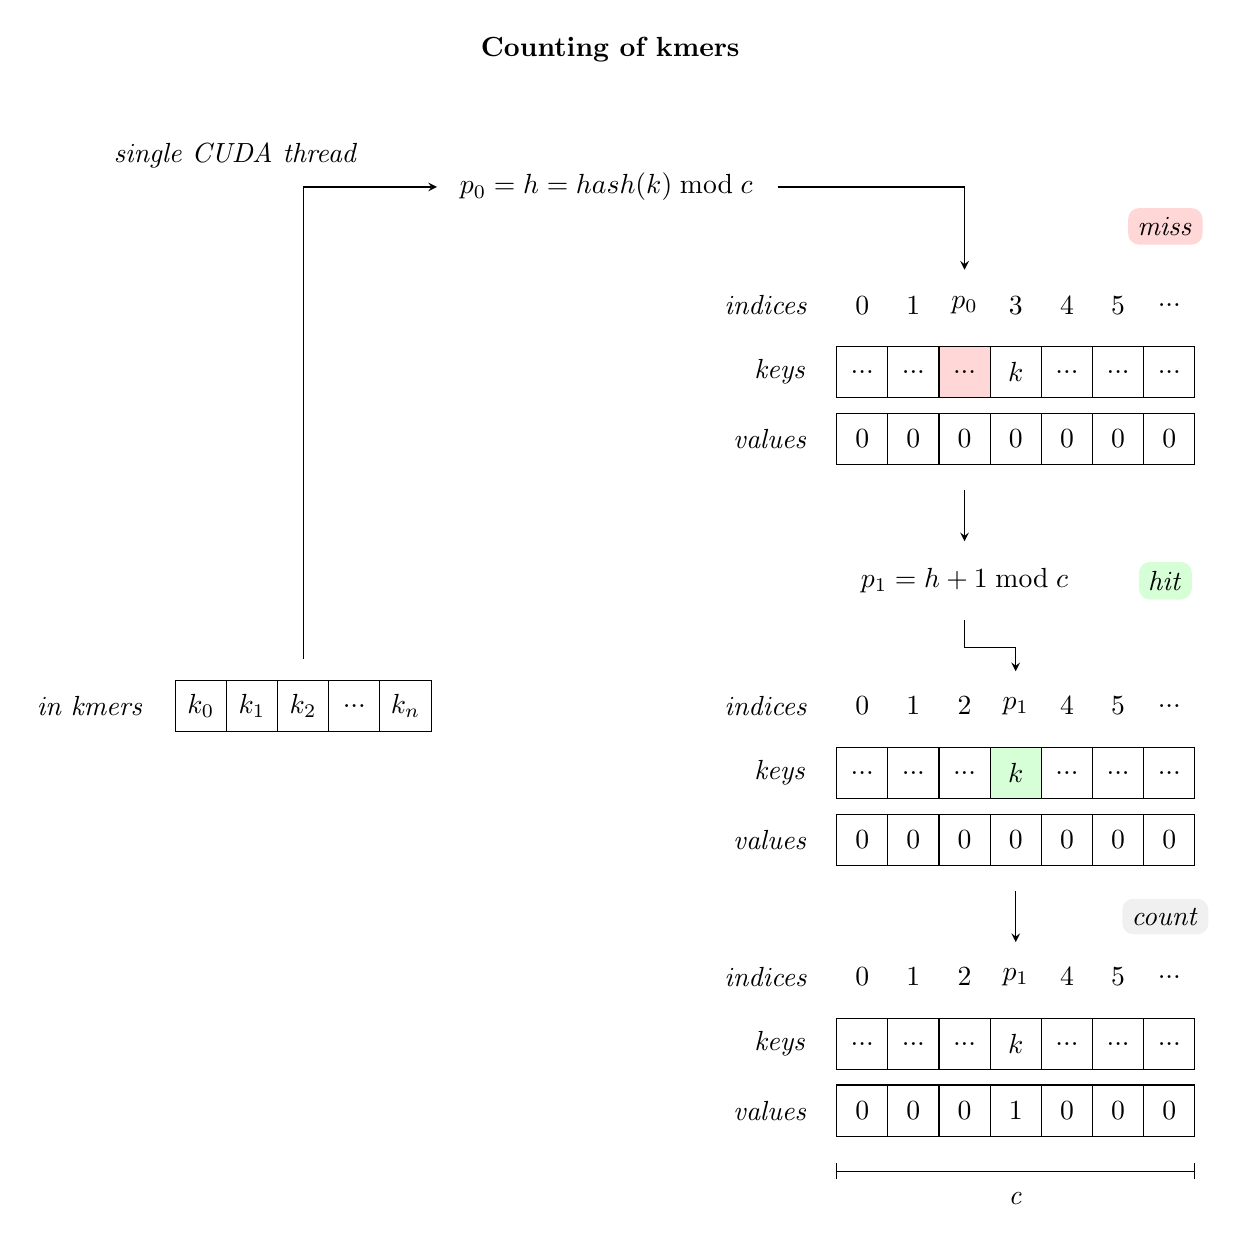
\begin{tikzpicture}

  \node at(1.2,0.75)[](thread){\smaller{\textbf{Counting of kmers}}};

  \node at(-5.4,-7.59)(kmers){\textit{\smaller{in kmers}}};

  \node at(-4,-7.59)[draw,minimum width=0.65cm,minimum height=0.65cm](){\smaller{$k_0$}};
  \node at(-3.35,-7.59)[draw,minimum width=0.65cm,minimum height=0.65cm](){\smaller{$k_1$}};
  \node at(-2.7,-7.59)[draw,minimum width=0.65cm,minimum height=0.65cm](){\smaller{$k_2$}};
  \node at(-2.05,-7.59)[draw,minimum width=0.65cm,minimum height=0.65cm](){\smaller{$...$}};
  \node at(-1.4,-7.59)[draw,minimum width=0.65cm,minimum height=0.65cm](){\smaller{$k_n$}};

  \node at(-3.55,-0.6)[](thread){\smaller{\textit{single CUDA thread}}};
  \draw [](-2.7,-6.99) -- (-2.7,-1);
  \draw [-stealth](-2.7,-1) -- (-1,-1);

  \node at(1.15,-1)(hash){\smaller{\textit{$p_0=h=hash(k) \bmod c$}}};

  \draw [](3.325,-1) -- (5.7,-1);
  \draw [-stealth](5.7,-1) -- (5.7,-2.05);

  \node at(8.25,-1.5)[fill=misscolor,rounded corners](miss){\textit{\smaller{miss}}};

  \node at(3.185,-2.5)(indices){\textit{\smaller{indices}}};
  \node at(3.365,-3.35)(keys){\textit{\smaller{keys}}};
  \node at(3.2375,-4.2)(values){\textit{\smaller{values}}};

  \node at(4.4,-2.5)[minimum width=0.65cm,minimum height=0.65cm](){\smaller{$0$}};
  \node at(5.05,-2.5)[minimum width=0.65cm,minimum height=0.65cm](){\smaller{$1$}};
  \node at(5.7,-2.5)[minimum width=0.65cm,minimum height=0.65cm](){\smaller{$p_0$}};
  \node at(6.35,-2.5)[minimum width=0.65cm,minimum height=0.65cm](){\smaller{$3$}};
  \node at(7,-2.5)[minimum width=0.65cm,minimum height=0.65cm](){\smaller{$4$}};
  \node at(7.65,-2.5)[minimum width=0.65cm,minimum height=0.65cm](){\smaller{$5$}};
  \node at(8.3,-2.5)[minimum width=0.65cm,minimum height=0.65cm](){\smaller{$...$}};

  \node at(4.4,-3.35)[draw,minimum width=0.65cm,minimum height=0.65cm](){\smaller{$...$}};
  \node at(5.05,-3.35)[draw,minimum width=0.65cm,minimum height=0.65cm](){\smaller{$...$}};
  \node at(5.7,-3.35)[draw,minimum width=0.65cm,minimum height=0.65cm,fill=misscolor](){\smaller{$...$}};
  \node at(6.35,-3.35)[draw,minimum width=0.65cm,minimum height=0.65cm](){\smaller{$k$}};
  \node at(7,-3.35)[draw,minimum width=0.65cm,minimum height=0.65cm](){\smaller{$...$}};
  \node at(7.65,-3.35)[draw,minimum width=0.65cm,minimum height=0.65cm](){\smaller{$...$}};
  \node at(8.3,-3.35)[draw,minimum width=0.65cm,minimum height=0.65cm](){\smaller{$...$}};

  \node at(4.4,-4.2)[draw,minimum width=0.65cm,minimum height=0.65cm](){\smaller{$0$}};
  \node at(5.05,-4.2)[draw,minimum width=0.65cm,minimum height=0.65cm](){\smaller{$0$}};
  \node at(5.70,-4.2)[draw,minimum width=0.65cm,minimum height=0.65cm](){\smaller{$0$}};
  \node at(6.35,-4.2)[draw,minimum width=0.65cm,minimum height=0.65cm](){\smaller{$0$}};
  \node at(7,-4.2)[draw,minimum width=0.65cm,minimum height=0.65cm](){\smaller{$0$}};
  \node at(7.65,-4.2)[draw,minimum width=0.65cm,minimum height=0.65cm](){\smaller{$0$}};
  \node at(8.3,-4.2)[draw,minimum width=0.65cm,minimum height=0.65cm](){\smaller{$0$}};

  \draw [-stealth](5.7,-4.85) -- (5.7,-5.5);

  \node at(5.7,-6)(hash){\smaller{\textit{$p_1=h+1 \bmod c$}}};

  \draw [](5.7,-6.5) -- (5.7,-6.85);
  \draw [](5.7,-6.85) -- (6.35,-6.85);
  \draw [-stealth](6.35,-6.85) -- (6.35,-7.15);

  \node at(8.25,-6)[fill=hitcolor,rounded corners](hit){\textit{\smaller{hit}}};

  \node at(3.185,-7.59)(indices){\textit{\smaller{indices}}};
  \node at(3.365,-8.44)(keys){\textit{\smaller{keys}}};
  \node at(3.2375,-9.29)(values){\textit{\smaller{values}}};

  \node at(4.4,-7.59)[minimum width=0.65cm,minimum height=0.65cm](){\smaller{$0$}};
  \node at(5.05,-7.59)[minimum width=0.65cm,minimum height=0.65cm](){\smaller{$1$}};
  \node at(5.7,-7.59)[minimum width=0.65cm,minimum height=0.65cm](){\smaller{$2$}};
  \node at(6.35,-7.59)[minimum width=0.65cm,minimum height=0.65cm](){\smaller{$p_1$}};
  \node at(7,-7.59)[minimum width=0.65cm,minimum height=0.65cm](){\smaller{$4$}};
  \node at(7.65,-7.59)[minimum width=0.65cm,minimum height=0.65cm](){\smaller{$5$}};
  \node at(8.3,-7.59)[minimum width=0.65cm,minimum height=0.65cm](){\smaller{$...$}};

  \node at(4.4,-8.44)[draw,minimum width=0.65cm,minimum height=0.65cm](){\smaller{$...$}};
  \node at(5.05,-8.44)[draw,minimum width=0.65cm,minimum height=0.65cm](){\smaller{$...$}};
  \node at(5.7,-8.44)[draw,minimum width=0.65cm,minimum height=0.65cm](){\smaller{$...$}};
  \node at(6.35,-8.44)[draw,minimum width=0.65cm,minimum height=0.65cm,fill=hitcolor](){\smaller{$k$}};
  \node at(7,-8.44)[draw,minimum width=0.65cm,minimum height=0.65cm](){\smaller{$...$}};
  \node at(7.65,-8.44)[draw,minimum width=0.65cm,minimum height=0.65cm](){\smaller{$...$}};
  \node at(8.3,-8.44)[draw,minimum width=0.65cm,minimum height=0.65cm](){\smaller{$...$}};

  \node at(4.4,-9.29)[draw,minimum width=0.65cm,minimum height=0.65cm](){\smaller{$0$}};
  \node at(5.05,-9.29)[draw,minimum width=0.65cm,minimum height=0.65cm](){\smaller{$0$}};
  \node at(5.70,-9.29)[draw,minimum width=0.65cm,minimum height=0.65cm](){\smaller{$0$}};
  \node at(6.35,-9.29)[draw,minimum width=0.65cm,minimum height=0.65cm](){\smaller{$0$}};
  \node at(7,-9.29)[draw,minimum width=0.65cm,minimum height=0.65cm](){\smaller{$0$}};
  \node at(7.65,-9.29)[draw,minimum width=0.65cm,minimum height=0.65cm](){\smaller{$0$}};
  \node at(8.3,-9.29)[draw,minimum width=0.65cm,minimum height=0.65cm](){\smaller{$0$}};

  \draw [-stealth](6.35,-9.94) -- (6.35,-10.59);

  \node at(8.25,-10.265)[fill=countcolor,rounded corners](count){\textit{\smaller{count}}};

  \node at(3.185,-11.03)(indices){\textit{\smaller{indices}}};
  \node at(3.365,-11.88)(keys){\textit{\smaller{keys}}};
  \node at(3.2375,-12.73)(values){\textit{\smaller{values}}};

  \node at(4.4,-11.03)[minimum width=0.65cm,minimum height=0.65cm](){\smaller{$0$}};
  \node at(5.05,-11.03)[minimum width=0.65cm,minimum height=0.65cm](){\smaller{$1$}};
  \node at(5.7,-11.03)[minimum width=0.65cm,minimum height=0.65cm](){\smaller{$2$}};
  \node at(6.35,-11.03)[minimum width=0.65cm,minimum height=0.65cm](){\smaller{$p_1$}};
  \node at(7,-11.03)[minimum width=0.65cm,minimum height=0.65cm](){\smaller{$4$}};
  \node at(7.65,-11.03)[minimum width=0.65cm,minimum height=0.65cm](){\smaller{$5$}};
  \node at(8.3,-11.03)[minimum width=0.65cm,minimum height=0.65cm](){\smaller{$...$}};

  \node at(4.4,-11.88)[draw,minimum width=0.65cm,minimum height=0.65cm](){\smaller{$...$}};
  \node at(5.05,-11.88)[draw,minimum width=0.65cm,minimum height=0.65cm](){\smaller{$...$}};
  \node at(5.7,-11.88)[draw,minimum width=0.65cm,minimum height=0.65cm](){\smaller{$...$}};
  \node at(6.35,-11.88)[draw,minimum width=0.65cm,minimum height=0.65cm](){\smaller{$k$}};
  \node at(7,-11.88)[draw,minimum width=0.65cm,minimum height=0.65cm](){\smaller{$...$}};
  \node at(7.65,-11.88)[draw,minimum width=0.65cm,minimum height=0.65cm](){\smaller{$...$}};
  \node at(8.3,-11.88)[draw,minimum width=0.65cm,minimum height=0.65cm](){\smaller{$...$}};

  \node at(4.4,-12.73)[draw,minimum width=0.65cm,minimum height=0.65cm](){\smaller{$0$}};
  \node at(5.05,-12.73)[draw,minimum width=0.65cm,minimum height=0.65cm](){\smaller{$0$}};
  \node at(5.70,-12.73)[draw,minimum width=0.65cm,minimum height=0.65cm](){\smaller{$0$}};
  \node at(6.35,-12.73)[draw,minimum width=0.65cm,minimum height=0.65cm](){\smaller{$1$}};
  \node at(7,-12.73)[draw,minimum width=0.65cm,minimum height=0.65cm](){\smaller{$0$}};
  \node at(7.65,-12.73)[draw,minimum width=0.65cm,minimum height=0.65cm](){\smaller{$0$}};
  \node at(8.3,-12.73)[draw,minimum width=0.65cm,minimum height=0.65cm](){\smaller{$0$}};

  \draw [](4.075,-13.5) -- (8.625,-13.5);
  \draw [](4.075,-13.4) -- (4.075,-13.6);
  \draw [](8.625,-13.4) -- (8.625,-13.6);
  \node at(6.35,-13.85)(c){\smaller{\textit{c}}};

\end{tikzpicture}
}
\caption{As an array of 64-bit integer encoded kmers are counted by the hash table, each CUDA thread will compute the first probe position $p_0$ for each individual kmer, and then continue probing by linearly moving up to the next consecutive slot until either an empty slot or the original kmer handled by the thread is observed. If en empty slot is observed, the thread terminates. If the original kmer is observed, the value at the current slot is increased.}
\label{figure:cucounter_hashtable_probing}
\end{center}
\end{figure}

